%======================================================================
% University of Waterloo Thesis Template for LaTeX 
% Last Updated August 2022
% by IST Client Services, 
% University of Waterloo, 200 University Ave. W., Waterloo, Ontario, Canada
% FOR ASSISTANCE, please send mail to helpdesk@uwaterloo.ca

% DISCLAIMER
% To the best of our knowledge, this template satisfies the current uWaterloo thesis requirements.
% However, it is your responsibility to assure that you have met all requirements of the University and your particular department.

% Many thanks for the feedback from many graduates who assisted the development of this template.
% Also note that there are explanatory comments and tips throughout this template.
%======================================================================
% Some important notes on using this template and making it your own...

% The University of Waterloo has required electronic thesis submission since October 2006. 
% See the uWaterloo thesis regulations at
% https://uwaterloo.ca/graduate-studies/thesis.
% This thesis template is geared towards generating a PDF version optimized for viewing on an electronic display, including hyperlinks within the PDF.

% DON'T FORGET TO ADD YOUR OWN NAME AND TITLE in the "hyperref" package configuration below. 
% Search for: PDFTITLE, PDFAUTHOR, PDFSUBJECT, and PDFKEYWORDS.
% THIS INFORMATION GETS EMBEDDED IN THE FINAL PDF DOCUMENT.
% You can view the information if you view properties of the PDF document.

% Many faculties/departments also require one or more printed copies. 
% This template attempts to satisfy both types of output. 
% See additional notes below.
% It is based on the standard "book" document class which provides all necessary sectioning structures and allows multi-part theses.

% If you are using this template in Overleaf (cloud-based collaboration service), then it is automatically processed and previewed for you as you edit.

% For people who prefer to install their own LaTeX distributions on their own computers, and process the source files manually, the following notes provide the sequence of tasks:
 
% E.g. to process a thesis called "mythesis.tex" based on this template, run:

% pdflatex mythesis	-- first pass of the pdflatex processor
% bibtex mythesis	-- generates bibliography from .bib data file(s)
% makeindex         -- should be run only if an index is used 
% pdflatex mythesis	-- fixes numbering in cross-references, bibliographic references, glossaries, index, etc.
% pdflatex mythesis	-- it takes a couple of passes to completely process all cross-references

% If you use the recommended LaTeX editor, Texmaker, you would open the mythesis.tex file, then click the PDFLaTeX button. Then run BibTeX (under the Tools menu).
% Then click the PDFLaTeX button two more times. 
% If you have an index as well,you'll need to run MakeIndex from the Tools menu as well, before running pdflatex
% the last two times.

% N.B. The "pdftex" program allows graphics in the following formats to be included with the "\includegraphics" command: PNG, PDF, JPEG, TIFF
% Tip: Generate your figures and photos in the size you want them to appear in your thesis, rather than scaling them with \includegraphics options.
% Tip: Any drawings you do should be in scalable vector graphic formats: SVG, PNG, WMF, EPS and then converted to PNG or PDF, so they are scalable in the final PDF as well.
% Tip: Photographs should be cropped and compressed so as not to be too large.

% To create a PDF output that is optimized for double-sided printing: 
% 1) comment-out the \documentclass statement in the preamble below, and un-comment the second \documentclass line.
% 2) change the value assigned below to the boolean variable "PrintVersion" from " false" to "true".

%======================================================================
%   D O C U M E N T   P R E A M B L E
% Specify the document class, default style attributes, and page dimensions, etc.
% For hyperlinked PDF, suitable for viewing on a computer, use this:
\documentclass[letterpaper,12pt,titlepage,oneside,final]{book}
 
% For PDF, suitable for double-sided printing, change the PrintVersion variable below to "true" and use this \documentclass line instead of the one above:
%\documentclass[letterpaper,12pt,titlepage,openright,twoside,final]{book}

% Some LaTeX commands I define for my own nomenclature.
% If you have to, it's easier to make changes to nomenclature once here than in a million places throughout your thesis!
\newcommand{\package}[1]{\textbf{#1}} % package names in bold text
\newcommand{\cmmd}[1]{\textbackslash\texttt{#1}} % command name in tt font 
\newcommand{\href}[1]{#1} % does nothing, but defines the command so the print-optimized version will ignore \href tags (redefined by hyperref pkg).
%\newcommand{\texorpdfstring}[2]{#1} % does nothing, but defines the command
% Anything defined here may be redefined by packages added below...

% This package allows if-then-else control structures.
\usepackage{ifthen}
\newboolean{PrintVersion}
\setboolean{PrintVersion}{false}
% CHANGE THIS VALUE TO "true" as necessary, to improve printed results for hard copies by overriding some options of the hyperref package, called below.

%\usepackage{nomencl} % For a nomenclature (optional; available from ctan.org)
\usepackage{amsmath,amssymb,amstext} % Lots of math symbols and environments
\usepackage[pdftex]{graphicx} % For including graphics N.B. pdftex graphics driver 
\usepackage{pgfplots}
\pgfplotsset{compat=1.18, width=14cm, height=10cm}
\usepgfplotslibrary{statistics}

% Hyperlinks make it very easy to navigate an electronic document.
% In addition, this is where you should specify the thesis title and author as they appear in the properties of the PDF document.
% Use the "hyperref" package 
% N.B. HYPERREF MUST BE THE LAST PACKAGE LOADED; ADD ADDITIONAL PKGS ABOVE
\usepackage[pdftex,pagebackref=false]{hyperref} % with basic options
%\usepackage[pdftex,pagebackref=true]{hyperref}
		% N.B. pagebackref=true provides links back from the References to the body text. This can cause trouble for printing.
\hypersetup{
    plainpages=false,       % needed if Roman numbers in frontpages
    unicode=false,          % non-Latin characters in Acrobat’s bookmarks
    pdftoolbar=true,        % show Acrobat’s toolbar?
    pdfmenubar=true,        % show Acrobat’s menu?
    pdffitwindow=false,     % window fit to page when opened
    pdfstartview={FitH},    % fits the width of the page to the window
%    pdftitle={uWaterloo\ LaTeX\ Thesis\ Template},    % title: CHANGE THIS TEXT!
%    pdfauthor={Author},    % author: CHANGE THIS TEXT! and uncomment this line
%    pdfsubject={Subject},  % subject: CHANGE THIS TEXT! and uncomment this line
%    pdfkeywords={keyword1} {key2} {key3}, % list of keywords, and uncomment this line if desired
    pdfnewwindow=true,      % links in new window
    colorlinks=true,        % false: boxed links; true: colored links
    linkcolor=blue,         % color of internal links
    citecolor=green,        % color of links to bibliography
    filecolor=magenta,      % color of file links
    urlcolor=cyan           % color of external links
}
\ifthenelse{\boolean{PrintVersion}}{   % for improved print quality, change some hyperref options
\hypersetup{	% override some previously defined hyperref options
%    colorlinks,%
    citecolor=black,%
    filecolor=black,%
    linkcolor=black,%
    urlcolor=black}
}{} % end of ifthenelse (no else)

\usepackage[automake,toc,abbreviations]{glossaries-extra} % Exception to the rule of hyperref being the last add-on package
% If glossaries-extra is not in your LaTeX distribution, get it from CTAN (http://ctan.org/pkg/glossaries-extra), 
% although it's supposed to be in both the TeX Live and MikTeX distributions. There are also documentation and 
% installation instructions there.


% Setting up the page margins...
% uWaterloo thesis requirements specify a minimum of 1 inch (72pt) margin at the
% top, bottom, and outside page edges and a 1.125 in. (81pt) gutter margin (on binding side). 
% While this is not an issue for electronic viewing, a PDF may be printed, and so we have the same page layout for both printed and electronic versions, we leave the gutter margin in.
% Set margins to minimum permitted by uWaterloo thesis regulations:
\setlength{\marginparwidth}{0pt} % width of margin notes
% N.B. If margin notes are used, you must adjust \textwidth, \marginparwidth
% and \marginparsep so that the space left between the margin notes and page
% edge is less than 15 mm (0.6 in.)
\setlength{\marginparsep}{0pt} % width of space between body text and margin notes
\setlength{\evensidemargin}{0.125in} % Adds 1/8 in. to binding side of all 
% even-numbered pages when the "twoside" printing option is selected
\setlength{\oddsidemargin}{0.125in} % Adds 1/8 in. to the left of all pages when "oneside" printing is selected, and to the left of all odd-numbered pages when "twoside" printing is selected
\setlength{\textwidth}{6.375in} % assuming US letter paper (8.5 in. x 11 in.) and side margins as above
\raggedbottom

% The following statement specifies the amount of space between paragraphs. Other reasonable specifications are \bigskipamount and \smallskipamount.
\setlength{\parskip}{\medskipamount}

% The following statement controls the line spacing.  
% The default spacing corresponds to good typographic conventions and only slight changes (e.g., perhaps "1.2"), if any, should be made.
\renewcommand{\baselinestretch}{1} % this is the default line space setting

% By default, each chapter will start on a recto (right-hand side) page.
% We also force each section of the front pages to start on a recto page by inserting \cleardoublepage commands.
% In many cases, this will require that the verso (left-hand) page be blank, and while it should be counted, a page number should not be printed.
% The following statements ensure a page number is not printed on an otherwise blank verso page.
\let\origdoublepage\cleardoublepage
\newcommand{\clearemptydoublepage}{%
  \clearpage{\pagestyle{empty}\origdoublepage}}
\let\cleardoublepage\clearemptydoublepage


%======================================================================
%   L O G I C A L    D O C U M E N T
% The logical document contains the main content of your thesis.
% Being a large document, it is a good idea to divide your thesis into several files, each one containing one chapter or other significant chunk of content, so you can easily shuffle things around later if desired.
%======================================================================
\begin{document}

%----------------------------------------------------------------------
% FRONT MATERIAL
% title page,declaration, borrowers' page, abstract, acknowledgements,
% dedication, table of contents, list of tables, list of figures, nomenclature, etc.
%----------------------------------------------------------------------
% T I T L E   P A G E
% -------------------
% Last updated August 16, 2022, by IST-Client Services
% The title page is counted as page `i' but we need to suppress the
% page number. Also, we don't want any headers or footers.
\pagestyle{empty}
\pagenumbering{roman}

% The contents of the title page are specified in the "titlepage"
% environment.
\begin{titlepage}
        \begin{center}
        \vspace*{1.0cm}

        \Huge
        {\bf Two Variable Analysis between Height and Heart Rate  }

        \vspace*{1.0cm}

        \normalsize
        by \\

        \vspace*{1.0cm}

        \Large
        Andy Yan and Alexandru Darie \\

        \vspace*{3.0cm}

        \normalsize
        A thesis \\
        presented to Mr. Wang \\ 
        in fulfillment of the \\
        culminating project for \\
        the completion of the Data Management Course\\
        at A.Y Jackson Secondary School\\

        \vspace*{2.0cm}

       North York, Ontario, Canada, 2022 \\

        \vspace*{1.0cm}

        \copyright\ Andy Yan and Alexandru Darie 2022 \\
        \end{center}
\end{titlepage}

% The rest of the front pages should contain no headers and be numbered using Roman numerals starting with `ii'
\pagestyle{plain}
\setcounter{page}{2}

\cleardoublepage % Ends the current page and causes all figures and tables that have so far appeared in the input to be printed.
% In a two-sided printing style, it also makes the next page a right-hand (odd-numbered) page, producing a blank page if necessary.
\phantomsection    % allows hyperref to link to the correct page
% D E C L A R A T I O N   P A G E
% -------------------------------
  % The following is a sample Declaration Page as provided by the GSO
  % December 13th, 2006.  It is designed for an electronic thesis.
 \addcontentsline{toc}{chapter}{Author's Declaration}
 \begin{center}\textbf{Author's Declaration}\end{center}
  
 \noindent
We hereby declare that we are the sole authors of this thesis. This is a true copy of the thesis, including any required final revisions, as accepted by our examiners. 

  \bigskip
  
  \noindent
We understand that our thesis may be made electronically available to the public.

\cleardoublepage
\phantomsection    % allows hyperref to link to the correct page

% A B S T R A C T
% ---------------
\addcontentsline{toc}{chapter}{Abstract}
\begin{center}\textbf{Abstract}\end{center}

Height and heart rate are two variables that play a significant role in the health industry. Comparing the two can provide useful information that can improve the products used in the industry and our daily lives. This data can also bring helpful contributions to the sports and athletics industry.

Throughout this report, there will be tables and graphs of conducted surveys used to collect the heights and heart rates of 50 male 17-year-old boys and 50 female 17-year-old girls. Using this data, we were able to come up with mathematical relationships that link our data and prove our hypothesis of the assumed relationship.

\cleardoublepage
\phantomsection    % allows hyperref to link to the correct page

% A C K N O W L E D G E M E N T S
% -------------------------------
\addcontentsline{toc}{chapter}{Acknowledgements}
\begin{center}\textbf{Acknowledgements}\end{center}

We would like to thank Overleaf for allowing us to create this beautiful document.
\cleardoublepage
\phantomsection    % allows hyperref to link to the correct page

% T A B L E   O F   C O N T E N T S
% ---------------------------------
\renewcommand\contentsname{Table of Contents}
\tableofcontents
\cleardoublepage
\phantomsection    % allows hyperref to link to the correct page

% L I S T   O F   F I G U R E S
% -----------------------------
\addcontentsline{toc}{chapter}{List of Figures}
\listoffigures



\cleardoublepage
\phantomsection		% allows hyperref to link to the correct page

% L I S T   O F   T A B L E S
% ---------------------------
\addcontentsline{toc}{chapter}{List of Tables}
\listoftables



\cleardoublepage
\phantomsection		% allows hyperref to link to the correct page

% C A L C U L A T I O N S
% ---------------------------
\addcontentsline{toc}{chapter}{Calculations}

{\huge \textbf{Calculations}}

\vspace*{1.0cm}

{\large Calculating the \textbf{Average} of the Data (males):}
\begin{equation}
\mu = 
\frac{
  \displaystyle\sum\limits_{k=1}^{50} x_{k}
}{50} = 81.44  , \hspace{0.5cm}
\fbox{\mu = 81.44} \label{1} 
\end{equation} 

{\large Calculating the \textbf{Standard Deviation} of the Data (males):}
\begin{equation}
\sigma = 
\sqrt{\frac{
  \displaystyle\sum\limits_{k=1}^{N} (x_{k} - \mu)^2
}{N-1}} = 
\sqrt{\frac{
  \displaystyle\sum\limits_{k=1}^{50} (x_{k} - 81.44)^2
}{49}} \approx 7.7648  , \hspace{0.5cm}
\fbox{\sigma = 7.7648} \label{2}
\end{equation} 

{\large Calculating the \textbf{Variance} of the Data (males):}
\begin{equation}
\sigma^2 = 7.7648^2 \approx 60.2921  , \hspace{0.5cm}
\fbox{\sigma^2 = 60.2921} \label{3}
\end{equation} 

{\large Calculating the \textbf{Pearson's R} of the Data (males):}
\begin{equation}
r = \frac{n\displaystyle\sum\limits_{i=1}^{50}x_i y_i - (\displaystyle\sum\limits_{i=1}^{50} x_i)(\displaystyle\sum\limits_{i=1}^{50}y_i)}
{\sqrt{[(n\displaystyle\sum\limits_{i=1}^{50}x_i^2) - (\displaystyle\sum\limits_{i=1}^{50}x_i)^2][(n\displaystyle\sum\limits_{i=1}^{50}y_i^2) - (\displaystyle\sum\limits_{i=1}^{50}y_i)^2]}} = 
\frac{2261.48}{\sqrt{(4253.22)(2954.32)}} = 0.638 \label{4}
\end{equation} 
\begin{equation}
\therefore \fbox{r = 0.638} \label{5}
\end{equation} 

\cleardoublepage

{\large Calculating the \textbf{Line of Best Fit} for the Data (males):}
\begin{equation}
a = \frac{n\displaystyle\sum\limits_{i=1}^{50}x_i y_i - (\displaystyle\sum\limits_{i=1}^{50} x_i)(\displaystyle\sum\limits_{i=1}^{50}y_i)}
{n(\displaystyle\sum\limits_{i=1}^{50}x_i^2) - (\displaystyle\sum\limits_{i=1}^{50}x_i)^2} = 
\frac{2261.48}{4253.22} \approx 0.5317 , \hspace{0.5cm} \therefore a = 0.5317 \label{6}
\end{equation} 
\begin{equation}
b = \overline{y} - a\overline{x} = 81.44 - 0.5317\cdot177.66 \approx -13.0236 , \hspace{0.5cm}              
 \therefore b = -13.0236 \label{7}
 \vspace{0.5cm}
\end{equation} 
\hspace{0.5cm} Therefore the Equation of the line of best fit is:
\begin{equation}
\fbox{y = 0.5317x - 13.0236} \label{8}
\end{equation}
\vspace{0.7cm}
\hline
\vspace{0.7cm}
 
%---------------------------------------------------------------------------------

{\large Calculating the \textbf{Average} of the Data (females):}
\begin{equation}
\mu = 
\frac{
  \displaystyle\sum\limits_{k=1}^{50} x_{k}
}{50} = 89.32  , \hspace{0.5cm}
\fbox{\mu = 89.32} \label{9}
\end{equation} 

{\large Calculating the \textbf{Standard Deviation} of the Data (females):}
\begin{equation}
\sigma = 
\sqrt{\frac{
  \displaystyle\sum\limits_{k=1}^{N} (x_{k} - \mu)^2
}{N-1}} = 
\sqrt{\frac{
  \displaystyle\sum\limits_{k=1}^{50} (x_{k} - 89.32)^2
}{49}} \approx 7.8101  , \hspace{0.5cm}
\fbox{\sigma = 7.8101} \label{10}
\end{equation} 

{\large Calculating the \textbf{Variance} of the Data (females):}
\begin{equation}
\sigma^2 = 7.8101^2 \approx 60.9977  , \hspace{0.5cm}
\fbox{\sigma^2 = 60.9977} \label{11}
\end{equation} 

{\large Calculating the \textbf{Pearson's R} of the Data (females):}
\begin{equation}
r = \frac{n\displaystyle\sum\limits_{i=1}^{50}x_i y_i - (\displaystyle\sum\limits_{i=1}^{50} x_i)(\displaystyle\sum\limits_{i=1}^{50}y_i)}
{\sqrt{[(n\displaystyle\sum\limits_{i=1}^{50}x_i^2) - (\displaystyle\sum\limits_{i=1}^{50}x_i)^2][(n\displaystyle\sum\limits_{i=1}^{50}y_i^2) - (\displaystyle\sum\limits_{i=1}^{50}y_i)^2]}} = 
\frac{1618.08}{\sqrt{(2233.78)(2988.88)}} = 0.6262 \label{12}
\end{equation} 
\begin{equation}
\therefore \fbox{r = 0.6262} \label{13}
\end{equation} 
\vspace{0.7cm}

{\large Calculating the \textbf{Line of Best Fit} for the Data (females):}
\begin{equation}
a = \frac{n\displaystyle\sum\limits_{i=1}^{50}x_i y_i - (\displaystyle\sum\limits_{i=1}^{50} x_i)(\displaystyle\sum\limits_{i=1}^{50}y_i)}
{n(\displaystyle\sum\limits_{i=1}^{50}x_i^2) - (\displaystyle\sum\limits_{i=1}^{50}x_i)^2} = 
\frac{1618.08}{2233.78} \approx 0.7244 , \hspace{0.5cm} \therefore a = 0.7244 \label{14}
\end{equation} 
\begin{equation}
b = \overline{y} - a\overline{x} = 89.32 - 0.7244\cdot169.62 \approx -33.5474 , \hspace{0.5cm}              
 \therefore b = -33.5474 \label{15}
 \vspace{0.5cm}
\end{equation} 
Therefore the Equation of the line of best fit is:
\begin{equation}
\fbox{y = 0.7244x - 33.5474} \label{16}
\end{equation}

\cleardoublepage

\phantomsection		% allows hyperref to link to the correct page

% Change page numbering back to Arabic numerals
\pagenumbering{arabic}

 

%----------------------------------------------------------------------
% MAIN BODY
% We suggest using a separate file for each chapter of your thesis.
% Start each chapter file with the \chapter command.
% Only use \documentclass or \begin{document} and \end{document} commands in this master document.
% Tip: Putting each sentence on a new line is a way to simplify later editing.
%----------------------------------------------------------------------
%======================================================================
\chapter{Introduction}
%======================================================================

Is there a correlation between one's height and heart rate? And if so would one's heart rate increase with height or the opposite? 

%----------------------------------------------------------------------
\section{Data Collection}
%----------------------------------------------------------------------

To research this topic, we collected data from primary sources by asking 50 17-year-old boys and girls from our school. We separated the data into boys and girls because girls tend to have varied heart rates from boys. We collected data in a way so that the distribution of height is well spread allowing us to concentrate on our topic. 

\section{Hypothesis}

Our hypothesis for this paper is: \textbf{the taller one is, the higher their heart rate should be.} We believe this because the larger one's body is, the more blood is needed to be pumped into the body which requires a higher heart rate.

\begin{table}[h]
    \section{General Data Analysis}
    \centering
    \caption{Main Data Part 1}
    \label{tab:table1}
\begin{tabular}{ cc }   % top level tables, with 2 columns
Males(Age 17)&\hspace{5em} Females(Age 17)\\  
% leftmost table of the top level table
\begin{tabular}{ ||c|c|| } 
\hline
Height(cm) & Heartbeat(bpm)\\ [0.5ex] 
\hline
\hline
163 & 75 \\
163 & 60 \\
164 & 75 \\
165 & 70 \\
165 & 72 \\
165 & 80 \\
166 & 75 \\
166 & 87 \\
167 & 79 \\
168 & 80 \\
168 & 76 \\
170 & 90 \\
170 & 70 \\
170 & 80 \\
171 & 69 \\
172 & 79 \\
172 & 92 \\
173 & 80 \\
173 & 76 \\
175 & 78 \\
175 & 87 \\
176 & 80 \\
176 & 85 \\
177 & 81 \\
178 & 81 \\
178 & 74 \\
\hline
\end{tabular} & \hspace{5em} % starting rightmost sub table
% table 2
\begin{tabular}{ ||c|c|| } 
\hline
Height(cm) & Heartbeat(bpm)\\ [0.5ex] 
\hline
\hline
160 & 69 \\
160 & 80 \\
160 & 80 \\
161 & 82 \\
162 & 90 \\
162 & 76 \\
162 & 84 \\
163 & 90 \\
163 & 85 \\
163 & 82 \\
163 & 100 \\
163 & 80 \\
163 & 96 \\
164 & 80 \\
164 & 86 \\
164 & 81 \\
165 & 72 \\
165 & 98 \\
165 & 86 \\
166 & 92 \\
166 & 82 \\
167 & 100 \\
168 & 89 \\
168 & 96 \\
168 & 85 \\
169 & 80 \\
\hline
\end{tabular} \\
\end{tabular}
\end{table}
\cleardoublepage

\begin{table}[h]
    \centering
    \caption{Main Data Part 2}
    \label{tab:table2}
\begin{tabular}{ cc }   % top level tables, with 2 columns
Males(Age 17) Continued&\hspace{5em} Females(Age 17) Continued\\  
% leftmost table of the top level table
\begin{tabular}{ ||c|c|| } 
\hline
Height(cm) & Heartbeat(bpm)\\ [0.5ex] 
\hline
\hline
180 & 68 \\
180 & 82 \\
180 & 84 \\
180 & 92 \\
181 & 91 \\
181 & 72 \\
181 & 76 \\
182 & 83 \\
182 & 76 \\
183 & 82 \\
183 & 83 \\
184 & 83 \\
185 & 84 \\
185 & 90 \\
186 & 88 \\
186 & 84 \\
188 & 90 \\
189 & 84 \\
190 & 86 \\
190 & 87 \\
193 & 92 \\
194 & 92 \\
195 & 95 \\
199 & 97 \\
\hline
\end{tabular} & \hspace{5em}  % starting rightmost sub table
% table 2
\begin{tabular}{ ||c|c|| } 
\hline
Height(cm) & Heartbeat(bpm)\\ [0.5ex] 
\hline
\hline
169 & 88 \\
170 & 90 \\
171 & 90 \\
172 & 92 \\
172 & 88 \\
172 & 92 \\
172 & 89 \\
173 & 91 \\
174 & 104 \\
174 & 89 \\
175 & 88 \\
175 & 96 \\
176 & 99 \\
176 & 91 \\
177 & 93 \\
178 & 94 \\
178 & 88 \\
178 & 97 \\
179 & 95 \\
180 & 97 \\
180 & 100 \\
181 & 100 \\
182 & 101 \\
183 & 93 \\
\hline
\end{tabular} \\
\end{tabular}
\end{table}
\\\\
To put the data into perspective, we will graph scatter plots with a line of best fit. 
\begin{minipage}[t]{0.5\textwidth}
\break 
\begin{center}
\break
    \textbf{Calculated Variables (Males)}
\end{center}
\[\mu = 81.44 \textbf{     (\ref{1})}\]
\[\sigma = 7.7648 \textbf{     (\ref{2})}\]
\[\sigma^2 = 60.2921 \textbf{     (\ref{3})}\]
\[r = 0.638 \textbf{     (\ref{5})}\]
\end{minipage}% % leave no gap
\begin{minipage}[t]{0.5\textwidth}
\break 
\begin{center}
\break
    \textbf{Calculated Variables (Females)}
\end{center}
\[\mu = 89.32 \textbf{     (\ref{9})}\]
\[\sigma = 7.8101 \textbf{     (\ref{10})}\]
\[\sigma^2 = 60.9977 \textbf{     (\ref{11})}\]
\[r = 0.6262 \textbf{     (\ref{12})}\]
\end{minipage}


\begin{figure}
    \caption{Scatter Plot Male}
    \label{fig:figure1l}
\end{figure}
\begin{tikzpicture}
\begin{axis}[
title = Height vs. Heartbeat in 17-year-old males,
xlabel={$Height(cm)$},
ylabel={$Heartbeat(bpm)$},
xmin = 160,xmax = 200,
ymax = 100,
]
\addplot+[
    only marks,
    scatter,
    mark size=2.9pt]
table[meta]
{data_male.txt};
]
\addplot[domain = 160:210, 
samples=100,
color=black,] {0.53171*x - 13.02362};

%ŷ = 0.53171X - 13.02362
\end{axis}
\end{tikzpicture}
\begin{center}
    \textbf{Line of Best Fit (Males):}
    \begin{equation}
    y = 0.5317x - 13.0236 \textbf{     (\ref{8})}
    \end{equation}
\end{center}
If we take a closer look at the graph, we can see that there is a moderate-to-strong positive linear correlation between the two variables being plotted. This is evident from the fact that the correlation coefficient (r) is equal to 0.638, which falls within the range of 0.50 to 0.70, which is indicative of a moderate-to-strong positive linear relationship. Upon further examination, we can also see that most of the data points tend to cluster around the line of best fit, which is a good indication that there is a strong relationship between the two variables being plotted. However, there are a few outliers that fall outside of the cluster, which could potentially indicate some variability or inconsistency in the data. Additionally, we can see that the highest heart rate in the data belongs to the tallest boy, and the lowest heart rate belongs to the shortest boy.


\begin{tikzpicture}
\begin{axis}[
title = Height vs. Heartbeat in 17-year-old females,
xlabel={$Height(cm)$},
ylabel={$Heartbeat(bpm)$},
xmin = 158,xmax = 184,
ymax = 105,
]
\addplot+[
    only marks,
    scatter,
    mark size=2.9pt]
table[meta]
{data_female.txt};
\addplot[domain = 158:184, 
samples=100,
color=black,] {0.72437*x - 33.54739};
]
\end{axis}
\end{tikzpicture}

\begin{figure}
    \caption{Scatter Plot Female}
    \label{fig:figure2}
\end{figure}
\begin{center}
    \textbf{Line of Best Fit (Females):}
    \begin{equation}
    y = 0.7244x - 33.5474 \textbf{     (\ref{16})}
    \end{equation}
\end{center}
Upon analyzing the graph for girls, we see that there is also a moderate-to-strong positive linear correlation between the two variables being plotted. This is evident from the fact that the correlation coefficient (r) is equal to 0.6262, which falls within the range of 0.50 to 0.70, indicating a moderate-to-strong positive linear relationship. From the graph, we can see that on the lower half most of the girls' heart-rates fall below the line of best fit, and the girls on the higher side fall on top.  
\\
\section{Grouped Data Analysis}
Grouped data analysis allows for more generalized height interval comparisons, helping us investigate the correlation.
\begin{center}
\begin{table}[h]
    \centering
    \caption{Grouped Heights}
    \label{tab:table3}
\end{table}
\vspace{0.5cm}
\\
\def\arraystretch{1}
{\setlength{\tabcolsep}{5em}
\begin{tabular}{|| c | c ||} 
\hline
\multicolumn{2}{||c||}{Grouped Frequency Distribution Table \textbf{Males}} \\
 \hline
 \hline
   Class Interval & Frequency\\ [0.5ex] 
 \hline
160 - 167 & 9\\
 \hline
168 - 175	& 12\\
 \hline
176 - 183	& 16\\
 \hline
184 - 191	& 9\\
 \hline
192 - 199	& 4\\
 \hline
  \textbf{Total:} & \textbf{50}\\
  \hline
\end{tabular}}
\end{center}

\begin{center}
\def\arraystretch{1}
{\setlength{\tabcolsep}{5em}
\begin{tabular}{|| c | c ||} 
\hline
\multicolumn{2}{||c||}{Grouped Frequency Distribution Table \textbf{Females}} \\
\hline
 \hline
   Class Interval & Frequency\\ [0.5ex] 
 \hline
160 - 164 & 16\\
 \hline
165 - 169	& 11\\
 \hline
170 - 174	& 9\\
 \hline
175 - 179	& 9\\
 \hline
180 - 184	& 5\\
 \hline
  \textbf{Total:} & \textbf{50}\\
  \hline
\end{tabular}}
\end{center}
\\\\
\\

\begin{table}[h]
    \centering
    \caption{Quartile Calculations}
    \label{tab:table4}
\end{table}

\begin{center}
    \begin{tabular}{ cc }   % top level tables, with 2 columns
    \def\arraystretch{1}
    \begin{tabular}{|| c | c | c | c | c | c ||}
    \hline
    \multicolumn{6}{||c||}{Male Quartile Calculations} \\
    \hline
    Interval & Q_1 & Q_2 & Q_3 & min & max\\
    \hline
    160-167 & 71 & 75 & 79.5 & 60 & 87\\ 
    168-175 & 76 & 79.5 & 83.5 & 69 & 92\\
    176-183 & 76 & 81.5 & 83.5 & 68 & 92\\
    184-191 & 84 & 86 & 89 & 83 & 90\\
    192-199 & 92 & 93.5 & 96 & 92 & 97\\
    \hline
    \end{tabular}
    
    \def\arraystretch{1}
    \begin{tabular}{|| c | c | c | c | c | c ||}
    \hline
    \multicolumn{6}{||c||}{Female Quartile Calculations} \\
    \hline
    Interval & Q_1 & Q_2 & Q_3 & min & max\\
    \hline
    160-164 & 80 & 82 & 88 & 69 & 100\\ 
    165-169 & 82 & 88 & 96 & 72 & 100\\
    170-174 & 89 & 90 & 92 & 88 & 104\\
    175-179 & 89.5 & 94 & 96.5 & 88 & 99\\
    180-184 & 95 & 100 & 100.5 & 93 & 101\\
    \hline
    \end{tabular}
\end{tabular}
\end{center}

\begin{figure}
    \centering
    \caption{Box Plots}
    \label{fig:figure2}
\end{figure}

\begin{center}
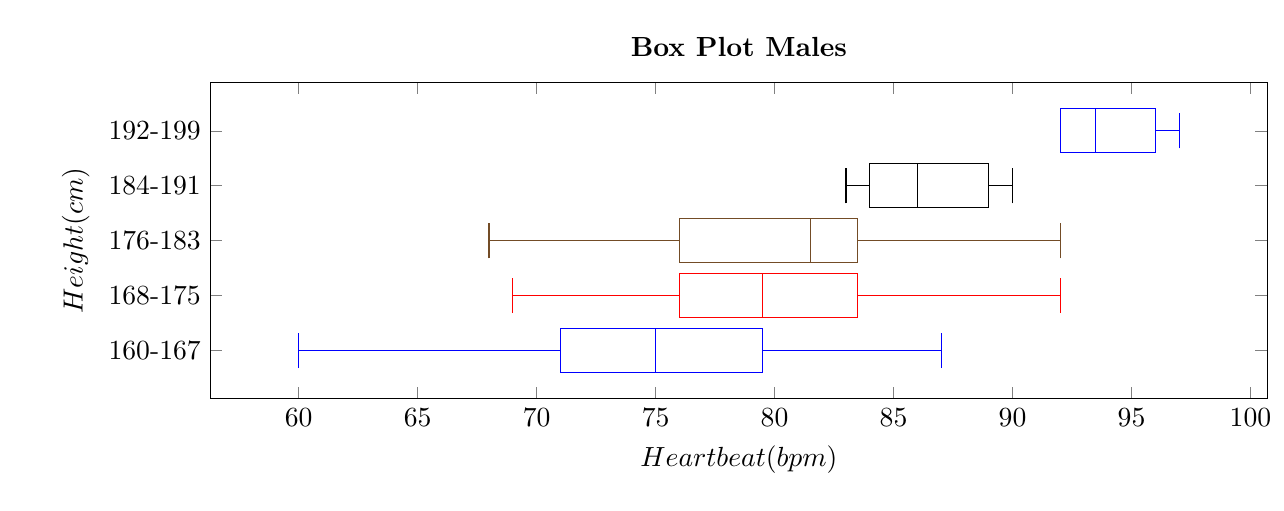
\begin{tikzpicture}
  \begin{axis}
    [
    title = \textbf{Box Plot Males},
    ytick={1,2,3,4,5},
    yticklabels={160-167, 168-175, 176-183, 184-191,192-199},
    ylabel={$Height(cm)$},
    xlabel={$Heartbeat(bpm)$},
    width=15cm,height=5.6cm,
    ]
    \addplot+[
    boxplot prepared={
      median=75,
      upper quartile=79.5,
      lower quartile=71,
      upper whisker=87,
      lower whisker=60
    },
    ] coordinates {};
    \addplot+[
    boxplot prepared={
      median=79.5,
      upper quartile=83.5,
      lower quartile=76,
      upper whisker=92,
      lower whisker=69
    },
    ] coordinates {};
    \addplot+[
    boxplot prepared={
      median=81.5,
      upper quartile=83.5,
      lower quartile=76,
      upper whisker=92,
      lower whisker=68
    },
    ] coordinates {};
    \addplot+[
    boxplot prepared={
      median=86,
      upper quartile=89,
      lower quartile=84,
      upper whisker=90,
      lower whisker=83
    },
    ] coordinates {};
    \addplot+[
    boxplot prepared={
      median=93.5,
      upper quartile=96,
      lower quartile=92,
      upper whisker=97,
      lower whisker=92
    },
    ] coordinates {};
  \end{axis}
\end{tikzpicture}

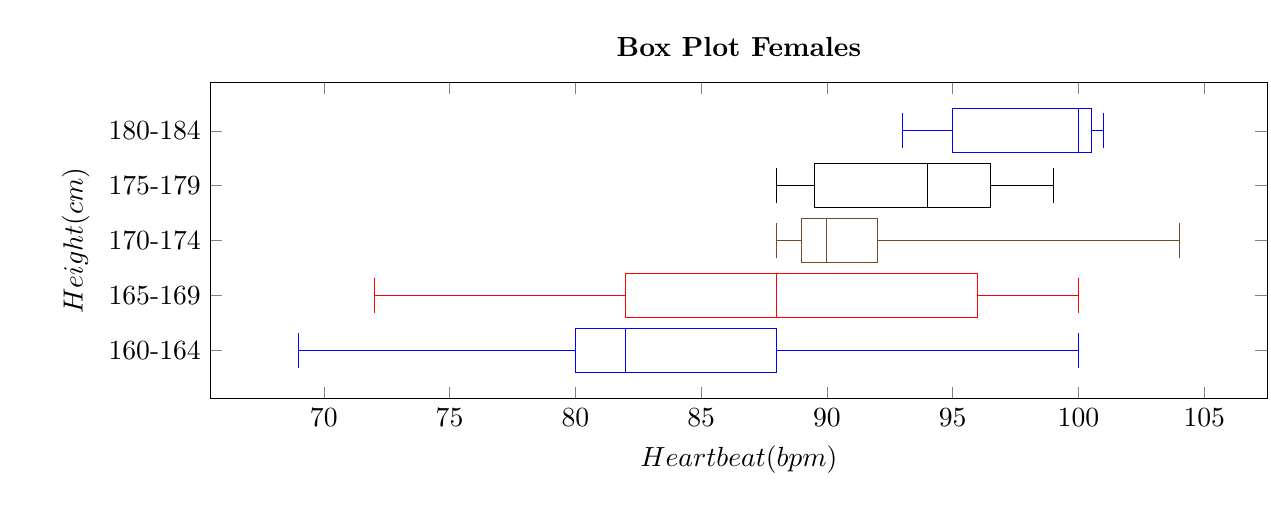
\begin{tikzpicture}
  \begin{axis}
    [
    title = \textbf{Box Plot Females},
    ytick={1,2,3,4,5},
    yticklabels={160-164, 165-169, 170-174, 175-179,180-184},
    ylabel={$Height(cm)$},
    xlabel={$Heartbeat(bpm)$},
    width=15cm,height=5.6cm,
    ]
    \addplot+[
    boxplot prepared={
      median=82,
      upper quartile=88,
      lower quartile=80,
      upper whisker=100,
      lower whisker=69
    },
    ] coordinates {};
    \addplot+[
    boxplot prepared={
      median=88,
      upper quartile=96,
      lower quartile=82,
      upper whisker=100,
      lower whisker=72
    },
    ] coordinates {};
    \addplot+[
    boxplot prepared={
      median=90,
      upper quartile=92,
      lower quartile=89,
      upper whisker=104,
      lower whisker=88
    },
    ] coordinates {};
    \addplot+[
    boxplot prepared={
      median=94,
      upper quartile=96.5,
      lower quartile=89.5,
      upper whisker=99,
      lower whisker=88
    },
    ] coordinates {};
    \addplot+[
    boxplot prepared={
      median=100,
      upper quartile=100.5,
      lower quartile=95,
      upper whisker=101,
      lower whisker=93
    },
    ] coordinates {};
  \end{axis}
\end{tikzpicture}

\end{center}
\\
\hspace{\parindent}A box plot is a useful tool for visualizing the distribution of a set of data and identifying any potential outliers. By analyzing our box plot, we can see that the majority of males have a heart rate between 70 beats per minute (bpm) and 85 bpm, while the majority of females have a heart rate between 85 bpm and 95 bpm. This is evident from the fact that the central boxes of the plots for each gender span these ranges, with the median heart rates falling near the center of the boxes. From both graphs, we can see that the majority of the data points are clustered within the mid-range of the heart rates, which suggests that there is a consistent relationship between the two variables being plotted.
%----------------------------------------------------------------------
%----------------------------------------------------------------------
%======================================================================
\chapter{Discussion}
%======================================================================

As seen throughout the introduction there seems to be a relationship that will be further discussed and analyzed in this section.

%----------------------------------------------------------------------
\section{Observations}
%----------------------------------------------------------------------
Firstly, the most evident observation to be made is: the average heart rate is increasing as the average height increases for this particular data set. Both correlations from males and females show a moderate-to-strong linear correlation due to both Pearson's R's  being very close to the boundary which shows a strong linear correlation (0.67). This statement is further supported by the box and whisker plots created.
Additionally, this proves the hypothesis to be true for this particular sample. In other words, for students in AY Jackson as height increases, heart rate also increases. 
\vspace{0.3cm}

Heart rate in this research experiment is labelled as the dependent variable because if it was independent, then it would not make sense for one to be taller just because they have a faster heart rate. Therefore, height is the independent variable and heart rate is the dependent variable. For this reason, this relationship is not a reverse cause-and-effect. The only possible relationships that can be drawn from this data are cause-and-effect and presumed relationships. The reason this relationship is not just cause-and-effect is because of the size of the data that was dealt with. Since the data size was not very large, this relationship cannot be fully justified as cause-and-effect especially since this is not the size of an entire population. There also could be hidden variables which will be addressed in the reflection tab (section 2.2).

%----------------------------------------------------------------------
\section{Reflection}
%----------------------------------------------------------------------
To conduct this experiment, a primary source of data collection was used to gather all the data. With this being said since there were only 2 people working on the collection, the data was obtained from a sample. This sample consisted of 50 seventeen-year-old males, and 50 seventeen-year-old females from the AY Jackson Secondary School. Since this sample does not reflect an entire population of 17-year-old males and females in all of Ontario, a definite conclusion cannot be drawn for a population, but it can be drawn for the sample from which the data originated.
\vspace{0.3cm}

Some very important and crucial pieces of information that were taken into consideration during this statistical experiment are the 3 main hidden variables. The first variable that was also kept constant was the age of all the people who were interviewed. A person's heart rate can change with age, so for this reason, the surveyed group needed to all have the same age. This made data collection slightly more challenging, but the results were more accurate. Another hidden variable would be the elevation of where students live. This is an uncontrolled variable, but since the sample was chosen from AY Jackson Secondary School, all of the students live in a general area where elevation does not play a major role. This made it negligible for the chosen sample but must be considered for national and international applications. Finally, the most important hidden variable would be activity and fitness levels. Students who have high fitness levels will have lower heart rates than others, which can account for the variations seen in the heart rate data. Likewise, health conditions also have a high chance of affecting this data, so that needs to be taken into account as well. 
\vspace{0.3cm}

Overall, the results of this investigation prove to be fairly accurate due to the calculated Pearson's R and the careful and well-thought experimenting process. There was not much Bias that partook during the surveying since there were no leading or loaded questions. There were some non-response biases due to the voluntary response method of surveying, but for ethical and personal reasons forced participation cannot be used. 
\vspace{0.3cm}

To further improve this analysis, a more universal surveying process of data can be used to gather more data which will better fit the size of a population. This will lead to a definite resolution to this relationship. Another method of improving this research project is to have a more refined and detailed filtering system where activity levels, elevation levels, and health conditions are used as parameters to organize and group the data into sections that reflect these various different populations.
%----------------------------------------------------------------------
% END MATERIAL
% Bibliography, Appendices, Index, etc.
%----------------------------------------------------------------------

% Bibliography

% The following statement selects the style to use for references.  
% It controls the sort order of the entries in the bibliography and also the formatting for the in-text labels.
\bibliographystyle{plain}
% This specifies the location of the file containing the bibliographic information.  
% It assumes you're using BibTeX to manage your references (if not, why not?).
\cleardoublepage % This is needed if the "book" document class is used, to place the anchor in the correct page, because the bibliography will start on its own page.
% Use \clearpage instead if the document class uses the "oneside" argument
\phantomsection  % With hyperref package, enables hyperlinking from the table of contents to bibliography             
% The following statement causes the title "References" to be used for the bibliography section:
\renewcommand*{\bibname}{References}

% Add the References to the Table of Contents
\addcontentsline{toc}{chapter}{\textbf{References}}

\bibliography{uw-ethesis.bib}
% Tip: You can create multiple .bib files to organize your references. 
% Just list them all in the \bibliogaphy command, separated by commas (no spaces).

% The following statement causes the specified references to be added to the bibliography even if they were not cited in the text. 
% The asterisk is a wildcard that causes all entries in the bibliographic database to be included (optional).
\nocite{*}
%----------------------------------------------------------------------

% Appendices

% The \appendix statement indicates the beginning of the appendices.
\appendix
% Add an un-numbered title page before the appendices and a line in the Table of Contents
\addcontentsline{toc}{chapter}{APPENDICES}
% Appendices are just more chapters, with different labeling (letters instead of numbers).
\chapter[Programs Used]{Height Heart Rate Grouper}
\label{AppendixA}

\begin{verbatim}
#include <iostream>
#include <vector>
using namespace std;
int main(){
    int a,b;
    vector<int>v[200];
    for(int i = 0;i<50;i++){
        cin>>a>>b;
        v[a].push_back(b);//array index is independent variable
    }
    for(int i = 0;i<=199;i++){
        int sz = v[i].size();
        if(sz>0){
            cout<<i<<":   ";
        }
        for(int j : v[i]){
            cout<<j<<",";
        }
        if(sz>0){
            cout<<"\n";
        }
    }
    return 0;
}

\end{verbatim}
\end{document} % end of logical document
